\documentclass[wide,a4paper,titlepage,12pt] {article}
\usepackage{polski}
\usepackage[utf8]{inputenc}
\usepackage{listings}
\usepackage{float}
\usepackage{slashbox}
\usepackage[table]{xcolor}
\usepackage{graphicx,pdflscape}
\usepackage{placeins}


\title{Grafika komputerowa - projekt}
\author{Tymon Tobolski (181037)}

% Title page layout (fold)
\makeatletter
\renewcommand{\maketitle}{
\begin{titlepage}
  \begin{center}
    \vspace*{3cm}
    \LARGE \@title \par
    \vspace{2cm}
    \textit{\small Autor:}\par
    \normalsize \@author\par \normalsize
    \vspace{3cm}
    \textit{\small Prowadzący:}\par
    Dr inż. Tomasz Kapłon \par
    \vspace{2cm}
    Wydział Elektroniki\\ III rok\\ Pn TP 08.15 - 11.00\par
    \vspace{4cm}
    \small 9 stycznia 2012
  \end{center}
\end{titlepage}
}
\makeatother
  \lstset{
    language=c++,
    basicstyle=\ttfamily\scriptsize,
    numbers=left,
    numberstyle=\scriptsize,
    stepnumber=10,
    numbersep=9pt,
    showspaces=false,
    showstringspaces=false,
    showtabs=false,
    breaklines=true,
  }

\begin{document}
\maketitle
  \section{Cel projektu}
  \paragraph{}
  Celem projektu jest implementacja algorytmu rekursywnego śledzenia promieni (Recursive Ray Tracing).

  \section{Ray Tracing}
  \paragraph{}
  Ray Tracing jest techniką generowania fotorealistycznych obrazów scen 3D wykorzystującą analize odbitych promieni świetlnych trafiających do obserwatora.
  \paragraph{}
  Dla każdego punktu rzutni wyprowadza się promień pierwotny o początku w położeniu obserwatora. Dla każdego takiego promienia wyszukiwany jest najbliższy punkt przecięcia z obiektami znajdującymi sie na scenie. Następnie wyznaczana jest jasność w tym punkcie dla każdego źródła światła zgodnie z modelem oświetlnia Phonga. Kolejnym krokiem algorytmu jest określenie odbitych promieni wtórnych i wykonanie dla każdego takiego promienia opisanych wyżej operacji. Obliczenia koloru dla danego punktu rzutni kończy się w momencie, gdy promienie nie przecinają już żadnych innych obiektów, lub osiągniety został maksymalny poziom rekurencji.

  \section{Opis programu}
  \paragraph{}
  Pierwszym krokiem programu jest wczytanie danych opisująych scene z pliku tekstowego. Przykładowy plik opisu sceny znajduje się poniżej.
  \begin{verbatim}
dimensions 400 400
background 0.3 0.3 0.3
global 0.1 0.1 0.1
sphere 0.7   3.0    0.0  -5.0  0.8 0.2 0.0  0.7 1.0 0.0  0.2 0.1 0.2  40
sphere 0.7  -3.0    0.0  -5.0  0.8 0.2 0.0  0.7 1.0 0.0  0.2 0.1 0.2  40
sphere 2.0   0.0    0.0  -3.0  0.8 0.1 0.0  0.8 0.1 0.0  0.2 0.1 0.2  40
sphere 2.0   0.0   -5.0  -3.0  0.8 0.2 0.0  0.0 0.7 1.0  0.2 0.1 0.2  40
sphere 2.0   0.0    5.0  -3.0  0.8 0.2 0.0  0.0 0.7 1.0  0.2 0.1 0.2  40
sphere 2.0  -5.0    2.5  -3.0  0.8 0.2 0.0  0.0 0.7 1.0  0.2 0.1 0.2  40
sphere 2.0  -5.0   -2.5  -3.0  0.8 0.2 0.0  0.0 0.7 1.0  0.2 0.1 0.2  40
sphere 2.0   5.0   -2.5  -3.0  0.8 0.2 0.0  0.0 0.7 1.0  0.2 0.1 0.2  40
sphere 2.0   5.0    2.5  -3.0  0.8 0.2 0.0  0.0 0.7 1.0  0.2 0.1 0.2  40
source       0.0    0.0  15.0  0.2 0.2 0.2  0.4 0.4 0.4  0.2 0.2 0.2
source      -5.0    0.0  10.0  0.2 0.2 0.2  1.0 0.0 1.0  0.3 0.3 0.1
source       5.0    0.0  10.0  0.2 0.2 0.2  1.0 0.0 1.0  0.3 0.3 0.1
source       5.0    0.0  12.0  0.2 0.2 0.2  0.0 1.0 1.0  0.4 0.5 0.3
source      -5.0    0.0  12.0  0.2 0.2 0.2  0.0 1.0 1.0  0.4 0.5 0.3
  \end{verbatim}
  \paragraph{}
  Takie dane są wczytywane do programu i zapisywane w odpowiednich strukturach.

  \paragraph{}
  \lstinputlisting{1.cpp}


  \paragraph{}
  W celu eliminacji często powtarzanego kodu - w tym wypadku trójpowtórzeniowej pętli \texttt{for} - wprowadzone zostało makro \texttt{TRIPLE}:
  \paragraph{}
  \lstinputlisting{2.cpp}

  \paragraph{}
  Poniżej znajduje się funkcja \texttt{draw()}, która dla każdego punktu rzutni generuje promień pierwotny i wywołuje algorytm śledzenia promieni.
  \paragraph{}
  \lstinputlisting{3.cpp}

  \paragraph{}
  Funkcja \texttt{trace()} składa się z kilku etapów: sprawdzeniu czy promień przecina obiekt sceny, obliczeniu parametrów na podstaie modelu oświetlenia Phonga oraz rekurencyjne wywołanie funkcji \texttt{trace()} dla promienia odbitego.
  \paragraph{}
  \lstinputlisting{4.cpp}

  \paragraph{}
  Funkcja sprawdzająca przcięcie promienia z obiektem sceny (funkcja iteruje po wszystkich sferach):
  \paragraph{}
  \lstinputlisting{5.cpp}

  \paragraph{}
  Obliczenie koloru z modeu oświetlenia Phonga:
  \paragraph{}
  \lstinputlisting{6.cpp}

  \newpage
  \section{Uzyskane rezultaty}
  \paragraph{}
  Poniżej znajdują sie wyniki działania programu dla różnego maksymalnego poziomy rekurencji.

  \begin{figure}[h!]
    \begin{center}
      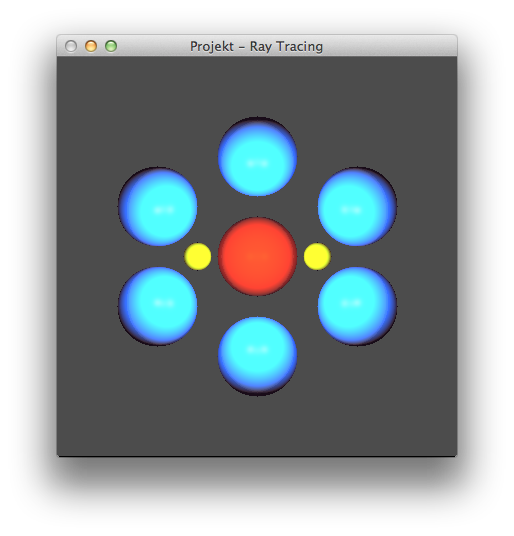
\includegraphics[width=\textwidth]{1.png}
      \caption{TRACE\_MAX = 1}
    \end{center}
  \end{figure}

  \begin{figure}[h!]
    \begin{center}
      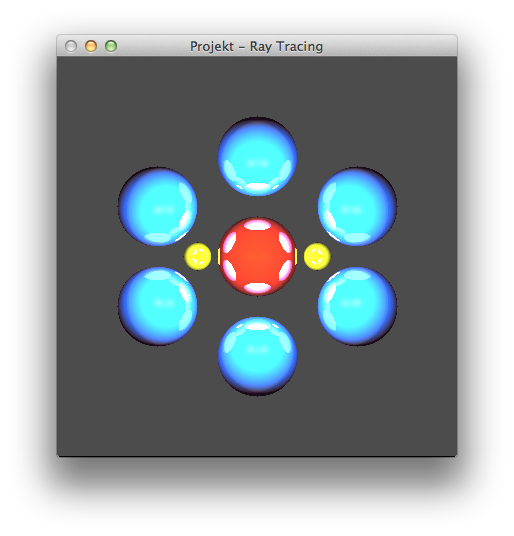
\includegraphics[width=\textwidth]{2.png}
      \caption{TRACE\_MAX = 2}
    \end{center}
  \end{figure}

  \begin{figure}[h!]
    \begin{center}
      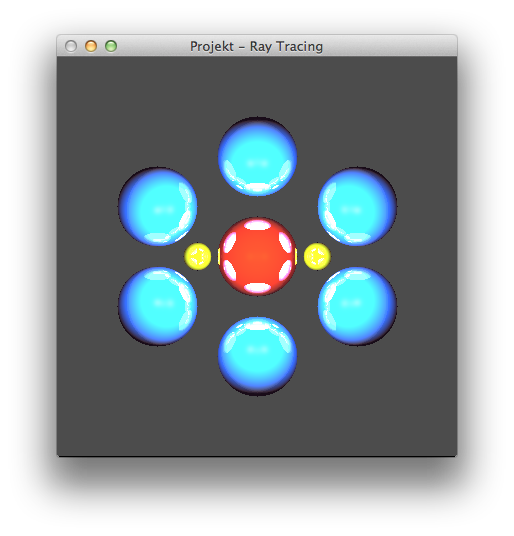
\includegraphics[width=\textwidth]{3.png}
      \caption{TRACE\_MAX = 3}
    \end{center}
  \end{figure}


  \newpage
  \paragraph{}
  Jak widać na rysunkach jeden poziom algorytmu Ray Tracing daje stosunkowo słabe rezultaty. Dodanie jednego poziomu rekurencji znacznie poprawia realizm oświetlenia sceny. Kolejny poziom nieznacznie poprawia wygląd odbić na powierzchni sfer.
  \paragraph{}
  Dla większych wartości maksymalnego poziomu rekurencji uzyskany obraz był identyczny co dla $TRACE\_MAX = 3$.

  \newpage
  \paragraph{}
  \newpage
  \section{Wnioski}
  \paragraph{}
  Algorytm rekursywnego śledzenia promieni pozwala na uzyskanie realistycznie oświetlonej sceny. Mimo uproszczonego modelu interakcji światła z otoczeniem metoda ta daje stosunkowo dobre rezultaty. Problemem może być wydajność algorytmu, który wymaga sporej ilości obliczeń. Ilość operacji jest zależna od rozdzielczości obrazu, liczby obiektów, a także ilości źródeł światła. Niebanalnym zadaniem jest też określenie czy promień przecina dany obiekt. W przypadku sfer sprowadza sie to do rozwiązania stosunkowo prostego równiania jednak przy barziej złożonych obiektach takie sprawdzenie może się okazać trudnych i czasochłonnym (zarówno dla programisty jak i procesora) zadaniem.


\end{document}